\documentclass[letterpaper, 11pt]{extarticle}
% ==================================================

% document parameters
% \usepackage[spanish, mexico, es-lcroman]{babel}
\usepackage[english]{babel}
\usepackage[margin = 1in]{geometry}

% ==================================================

% Packages for math
\usepackage{mathrsfs}
\usepackage{amsfonts}
\usepackage{amsmath}
\usepackage{amsthm}
\usepackage{amssymb}
\usepackage{physics}
\usepackage{dsfont}
\usepackage{esint}

% ==================================================

% Packages for writing
\usepackage{enumerate}
\usepackage[shortlabels]{enumitem}
\usepackage{framed}
\usepackage{csquotes}

% ==================================================

% Miscellaneous packages
\usepackage{todonotes}
\usepackage{float}
\usepackage{tabularx}
\usepackage{xcolor}
\usepackage{multicol}
\usepackage{subcaption}
\usepackage{caption}
\captionsetup{format = hang, margin = 10pt, font = small, labelfont = bf}

% Citation
\usepackage[round, authoryear]{natbib}

% Hyperlinks setup
\usepackage{hyperref}
\definecolor{links}{rgb}{0.36,0.54,0.66}
\hypersetup{
   colorlinks = true,
    linkcolor = black,
     urlcolor = blue,
    citecolor = blue,
    filecolor = blue,
    pdfauthor = {Author},
     pdftitle = {Title},
   pdfsubject = {subject},
  pdfkeywords = {one, two},
  pdfproducer = {LaTeX},
   pdfcreator = {pdfLaTeX},
   }
\usepackage{titlesec}
\usepackage[many]{tcolorbox}

% Adjust spacing after the chapter title
\titlespacing*{\chapter}{0cm}{-2.0cm}{0.50cm}
\titlespacing*{\section}{0cm}{0.50cm}{0.25cm}

% Indent 
\setlength{\parindent}{0pt}
\setlength{\parskip}{1ex}

% --- Theorems, lemma, corollary, postulate, definition ---
% \numberwithin{equation}{section}

\newtcbtheorem[]{problem}{Problema}%
    {enhanced,
    colback = black!5, %white,
    colbacktitle = black!5,
    coltitle = black,
    boxrule = 0pt,
    frame hidden,
    borderline west = {0.5mm}{0.0mm}{black},
    fonttitle = \bfseries\sffamily,
    breakable,
    before skip = 3ex,
    after skip = 3ex
}{problem}

\tcbuselibrary{skins, breakable}

% --- You can define your own color box. Just copy the previous \newtcbtheorm definition and use the colors of yout liking and the title you want to use.
% --- Basic commands ---
%   Euler's constant
\newcommand{\eu}{\mathrm{e}}

%   Imaginary unit
\newcommand{\im}{\mathrm{i}}

%   Sexagesimal degree symbol
\newcommand{\grado}{\,^{\circ}}

% --- Comandos para álgebra lineal ---
% Matrix transpose
\newcommand{\transpose}[1]{{#1}^{\mathsf{T}}}

%%% Comandos para cálculo
%   Definite integral from -\infty to +\infty
\newcommand{\Int}{\int\limits_{-\infty}^{\infty}}

%   Indefinite integral
\newcommand{\rint}[2]{\int{#1}\dd{#2}}

%  Definite integral
\newcommand{\Rint}[4]{\int\limits_{#1}^{#2}{#3}\dd{#4}}

%   Dot product symbol (use the command \bigcdot)
\makeatletter
\newcommand*\bigcdot{\mathpalette\bigcdot@{.5}}
\newcommand*\bigcdot@[2]{\mathbin{\vcenter{\hbox{\scalebox{#2}{$\m@th#1\bullet$}}}}}
\makeatother

%   Hamiltonian
\newcommand{\Ham}{\hat{\mathcal{H}}}

%   Trace
\renewcommand{\Tr}{\mathrm{Tr}}

% Christoffel symbol of the second kind
\newcommand{\christoffelsecond}[4]{\dfrac{1}{2}g^{#3 #4}(\partial_{#1} g_{#2 #4} + \partial_{#2} g_{#1 #4} - \partial_{#4} g_{#1 #2})}

% Riemann curvature tensor
\newcommand{\riemanncurvature}[5]{\partial_{#3} \Gamma_{#4 #2}^{#1} - \partial_{#4} \Gamma_{#3 #2}^{#1} + \Gamma_{#3 #5}^{#1} \Gamma_{#4 #2}^{#5} - \Gamma_{#4 #5}^{#1} \Gamma_{#3 #2}^{#5}}

% Covariant Riemann curvature tensor
\newcommand{\covariantriemanncurvature}[5]{g_{#1 #5} R^{#5}{}_{#2 #3 #4}}

% Ricci tensor
\newcommand{\riccitensor}[5]{g_{#1 #5} R^{#5}{}_{#2 #3 #4}}

\begin{document}

\begin{Huge}
    Cálculo II - \textsf{\textbf{Trabajo Grupal 2}} 
    
\end{Huge}

\vspace{2ex}

\textsf{\textbf{Integrantes:}} Grupo 2, ..., André V, ... \\
\textsf{\textbf{Carrera:}} \text{Ing. Informática - FCyT UMSS}


\vspace{2ex}

El trabajo plantea resolver la ecuación diferencial propuesta en \citep{TG2C2}, descrito a continuación. Así también se simula el comportamiento de una partícula para $t \in [0,2\pi]$ en GeoGebra \citep{geo}, describiendo los vectores tangente, normal, binormal unitarios (correspondientes al Triedro de Frenet), la curvatura y torsión.

\begin{problem}{EEDD}{}
 Resolver la ecuación diferencial:
\begin{equation}
    \frac{d^2r}{dt^2} = (-12\cos(3t)\sin(t)-20\cos(t)\sin(3t), 3\sin(t), -8\cos^2(2t)+8\sin^2(2t)) \quad t\in[0,2\pi]\label{eedd}
\end{equation}
Condición inicial $r(0) = (0, 0, 3)$ y $\frac{dr}{dt}(0) = (6, -3, 0)$
\end{problem}

Por tanto, se integró una vez a fin de obtener $r'(t)$ para evaluarla cuando $t=0$ y obtener el valor de las constantes; iterando este paso por segunda vez para obtener $r(t)$. Las ecuaciones \ref{e2}-\ref{e3} describen lo explicado. Para el cálculo, se utilizó la calc. TI-Nspire™ CX II CAS, en su función de ecuaciones diferenciales.

\begin{align}
r''(t)=\left\{\begin{matrix}
x''(t) &= -12\cos(3t)\sin(t)-20\cos(t)\sin(3t) \\
y''(t) &= 3\sin(t) \\
z''(t) &= -8\cos^2(2t)+8\sin^2(2t))
\end{matrix}\right., \quad t\in[0,2\pi] \label{e2} \\
r'(t)=\left\{\begin{matrix}
x'(t) = \int x''(t)dt =& 4\cos(4t)+2\cos(2t)+C_1 \\
y'(t) = \int y''(t)dt =& -3\cos(t)+C_2 \\
z'(t) = \int z''(t)dt =& -4\sin(2t)\cos(2t)+C_3
\end{matrix}\right., \quad t\in[0,2\pi]  \label{} \\
r'(0)=\left\{\begin{matrix}
x'(0) = 6 =& 4\cos(4(0))+2\cos(2(0))+C_1 &\implies C_1=0  \\
y'(0) = -3 =& -3\cos(0)+C_2 &\implies C_2=0\\
z'(0) = 0 =& -4\sin(2(0))\cos(2(0))+C_3 &\implies C_3=0
\end{matrix}\right. \label{} \\
r'(t)=(4\cos(4t)+2\cos(2t),-3\cos(t),-4\sin(2t)\cos(2t)), \quad t\in[0,2\pi] \label{}\\
r(t)=\left\{\begin{matrix}
x(t) = \int x'(t)dt =& \sin(4t)+\sin(2t)+C_4 \\
y(t) = \int y'(t)dt =& -3\sin(t)+C_5 \\
z(t) = \int z'(t)dt =& \cos^2(2t)+C_6
\end{matrix}\right., \quad t\in[0,2\pi]  \label{} \\
r(0)=\left\{\begin{matrix}
x(0) = 0 =& \sin(4(0))+\sin(2(0))+C_4 &\implies C_4=0  \\
y(0) = 0 =& -3\sin(0)+C_5 &\implies C_5=0\\
z(0) = 3 =& \cos^2(2(0))+C_6 &\implies C_6=2
\end{matrix}\right. \label{} \\
\boxed{r(t)=(\sin(4t)+\sin(2t),-3\sin(t),\cos^2(2t))+2, \quad t\in[0,2\pi]} \label{e3}
\end{align}

Con la EEDD ya resuelta se procedió a realizar la animación en GeoGebra.

\bigskip{\textit{\normalsize{Para el cálculo de esta curva, que nace a partir de la resolución de la ecuación diferencial planteada, se procede con los siguientes pasos para calcular y graficar dichos elementos en Geogebra:}}}

\begin{itemize}
    \item{\textbf{\underline{\normalsize{La Curva.-}}}}
        \smallskip{\normalsize{Para la graficación de la curva dada por el resultado del desarrollo de la ecuación diferencial, insertamos el siguiente código en Geogebra, respecto a la ec. \eqref{e3}:}}
        \begin{center}
            \begin{equation}
           r(t) = Curva((sen(4t) + sen(2t), -3sen(t), cos^{2}(2t) + 2), t\in[0, 2\pi])
        \end{equation}
        \end{center}
        
        \bigskip

    \item{\textbf{\underline{\normalsize{La 1° derivada de la curva [$v(t)$].-}}}}
    \smallskip{\normalsize{Para el cálculo y la graficación de la 1° derivada de la curva dada por el resultado del desarrollo de la ecuación diferencial, insertamos el siguiente código en Geogebra:}}

        \begin{center}
            \begin{equation}
            v(t) = Derivada(r(t)) = \quad
                \left.\begin{matrix}
                x &= 4\cos(4t)+2\cos(2t) \\
                y &= -3\cos(t) \\
                z &= 2*2\sin(2)(-1)\cos(2t)
                \end{matrix}\right\}0\leq t\leq 6.28
                \label{derivada1}
            \end{equation}
        \end{center}
    \bigskip
    
    \item{\textbf{\underline{\normalsize{La 2° Derivada de la Curva [$a(t)$].-}}}}
    \smallskip{\normalsize{Para el cálculo y la graficación de la 2° derivada de la curva dada por el resultado del desarrollo de la ecuación diferencial, insertamos el siguiente código en Geogebra, respecto a la ec. \eqref{derivada1}:}}
        \begin{center}
            \begin{equation}
                a(t) = Derivada(v(t), 2)
                \label{derivada2}
            \end{equation}   
        \end{center}
    \bigskip{\textit{Nota: La expresión derivada es demasiado larga para ser expresada en el documento, sin embargo en el archivo de Geogebra, se puede apreciar su cálculo efectuado}}
    \bigskip

    \item{\textbf{\underline{\normalsize{La 3° Derivada de la Curva [$c(t)$].-}}}}
    \smallskip{\normalsize{Para el cálculo y la graficación de la 2° derivada de la curva dada por el resultado del desarrollo de la ecuación diferencial, insertamos el siguiente código en Geogebra, respecto a la ec. \eqref{derivada2}:}}
        \begin{center}
            \begin{equation}
                c(t) = Derivada(a(t), 3)
            \end{equation}
        \end{center}
    \bigskip{\textit{Nota: Al igual que la segunda derivada, la tercera derivada es demasiado larga para ser expresada en el documento, sin embargo en el archivo de Geogebra, se puede apreciar su cálculo efectuado}}
    \bigskip

    \item{\textbf{\underline{\normalsize{El Vector Tangente [T].-}}}}
    \smallskip{\normalsize{Para el cálculo y la graficación del vector tangente en relación a la curva dada por el resultado del desarrollo de la ecuación diferencial, insertamos el siguiente código en Geogebra:}}
        \begin{center}
            \textit{Para obtener el cálculo del vector tangente, se toma en cuenta la 1° derivada de la curva, y se calcula la Norma de esta derivada, por medio de la siguiente ecuación:}
            \begin{equation}
                \left||v(t)\right|| =\sqrt{{v(t)^2}}
            \end{equation}

            \textit{Así mismo, con la Norma de la 1° derivada, calculada, procedemos al cálculo del vector Tangente, dado por la siguiente fórmula en Geogebra:}
            \begin{equation}
                T = Vector(\frac{v(t)}{\sqrt{v(t) * v(t)}})
            \end{equation}
        \end{center}
    \bigskip

    \item{\textbf{\underline{\normalsize{El Vector Binormal [B] y el Vector Normal [N].-}}}}
    \smallskip{\normalsize{Para el cálculo y la graficación del vector BInormal en relación a la curva dada por el resultado del desarrollo de la ecuación diferencial, insertamos el siguiente código en Geogebra:}}
        \begin{center}
            \textit{Para obtener el cálculo del vector binormal, se toma en cuenta el producto vectorial dado entre la 1° derivada y la 2° derivada de la curva, dividido entre la normal de dicho producto vectorial, elevado al cuadrado, calculado por medio de la siguiente ecuación:}
            \begin{equation}
                B=\frac{v(t) \times a(t)}{\left||v(t) \times a(t)\right||^2}
            \end{equation}
            \textit{Dada la ecuación del producto vectorial entre ambas derivadas, obtendremos el vector binormal, insertando el siguiente código en Geogebra:}
                \begin{equation}
                   B = Vector(\frac{v(t) \times a(t)}{\sqrt{(v(t) \times a(t)) * ((v(t) \times a(t))}})
                \end{equation}
    \end{center}
    \smallskip{\normalsize{Para el cálculo y la graficación del vector normal en relación a la curva dada por el resultado del desarrollo de la ecuación diferencial, insertamos el siguiente código en Geogebra:}}
        \begin{center}
            \textit{Para obtener el cálculo del vector normal, se toma en cuenta el producto vectorial dado entre los vectores: tangente y binormal, calculado por medio de la siguiente ecuación:}
            \begin{equation}
                N = B \times T
            \end{equation}
        \end{center}
    \bigskip

    \item{\textbf{\underline{\normalsize{La Curvatura [$\rho$].-}}}}
    \smallskip{\normalsize{Para el cálculo y la graficación de la curvatura en relación a la curva dada por el resultado del desarrollo de la ecuación diferencial, insertamos el siguiente código en Geogebra:}}
        \begin{center}
            \textit{Para calcular la curvatura que forma el desplazamiento del Triedro de Frenet y demás elementos sobre la función, utilizaremos la norma del producto vectorial entre la 1° y la 2° derivada, dividido entre la norma de la 1° derivada, elevada al cubo, dado que ya tenemos dichos elementos calculados, ingresaremos la fórmula al Geogebra, para el calculo de la curvatura, la cuál es:}
            \begin{equation}
                \rho = \frac{\sqrt{(v(t) \times a(t)) * (v(t) \times a(t))}}{(\sqrt{v(t) * v(t)})^{2}}
            \end{equation}
        \end{center}
    \bigskip

    \item{\textbf{\underline{\normalsize{La Torsión [$\tau$].-}}}}
    \smallskip{\normalsize{Para el cálculo y la graficación de la torsión en relación a la curva dada por el resultado del desarrollo de la ecuación diferencial, insertamos el siguiente código en Geogebra:}}
        \begin{center}
            \textit{Para calcular la torsión que genera el desplazamiento del Triedro de Frenet y demás elementos sobre la función, utilizaremos el producto vectorial entre la 1° y la 2° derivada, multiplicado por la 3° derivada, todo esto a su vez, está dividido entre la norma del producto vectorial entre la 1° y 2° derivada, elevada al cuadrado; dado que ya tenemos dichos elementos calculados, ingresaremos la fórmula al Geogebra, para el calculo de la curvatura, la cuál es:}
            \begin{equation}
                \tau = \frac{(v(t) \times a(t)) * c(t)}{(\sqrt{(v(t) \times a(t)) * (v(t) \times a(t))})^{3}}
            \end{equation}
        \end{center}
\end{itemize}

Se detalla una captura de la ejecución con lo explicado preciamente en la Fig. \ref{fig:enter-label}.

\begin{figure}[b!]
    \centering
    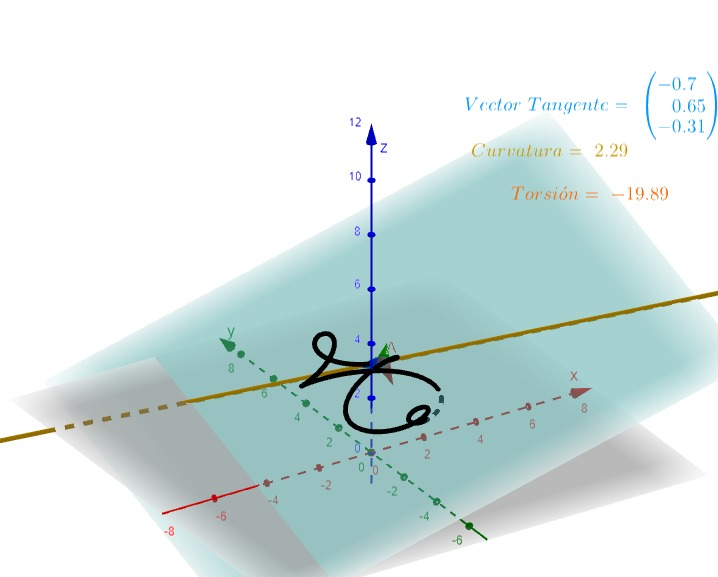
\includegraphics[width=6cm, height=8cm]{"media/comp.jpg"}
    \caption{Imagen sobre la gráfica de la Función, más sus componentes, la animación está disponible en \citep{geo}.}
    \label{fig:enter-label}
\end{figure}
% =================================================

\newpage

% \vfill

\bibliographystyle{plainnat}
\renewcommand{\refname}{Referencias}
\bibliography{references}

\end{document}